\documentclass[11pt]{report}

\usepackage{geometry}
\geometry{
	a4paper,
	top=3cm,
	bottom=3cm,
	left=3.5cm,
	right=2.5cm
}
\usepackage[charter]{mathdesign}
\usepackage{longtable}
\usepackage{graphics}
\usepackage{graphicx}
\usepackage{caption}
\usepackage{subcaption}
\usepackage{array}
\usepackage{float}
\usepackage{enumerate}
\usepackage{amsmath}
\usepackage{listings}
\usepackage{algorithm}
\usepackage[noend]{algpseudocode}
\usepackage{xcolor}
\usepackage[nottoc]{tocbibind}
\graphicspath{ {images/} }
\usepackage{titlesec}
\titleformat{\chapter}[display]   
{\normalfont\huge\bfseries}{\chaptertitlename\ \thechapter}{20pt}{\Huge}   
\titlespacing*{\chapter}{0pt}{-50pt}{45pt}

\lstset { %
	language=C++,
	%backgroundcolor=\color{black!5}, % set backgroundcolor
	basicstyle=\footnotesize,% basic font setting
}

%% Title Page
%\title{Computer Graphics(Sessional) -- CSE-458}
%\author{Muhammad Rabiul Alam\linebreak[2] (1204049)}
%\date{\parbox{\linewidth}{\centering%
%		\today\endgraf\bigskip
%		L-4, T-1. Group: A2\endgraf\medskip
%}}



\begin{document}
	\begin{titlepage}
		\begin{center}
			{\huge\bfseries Computer Graphics (Sessional)--CSE-458\\}
			% ----------------------------------------------------------------
			\vspace{1.5cm}
			{\Large\bfseries Muhammad Rabiul Alam}\\[5pt]
			1204049\\[14pt]
			L-4, T-II\\[14pt]
			Group: A2\\[14pt]
			% ----------------------------------------------------------------
			\vspace{2cm}
			{Submitted To} \\[8pt]
			\hspace{2.9cm}\textsc{\Large{{Farzana Yasmin\newline Lecturer, Department of CSE, CUET}}} \\[5pt]
			% {By}\\[5pt] {\Large \sc {Me}}
			
			\vfill
			{July 31, 2017}
			
			\vfill
			% ----------------------------------------------------------------
			{\bfseries Department of CSE}\\[11pt]
			{\bfseries Chittagong University of Engineering \& Technology}\\[11pt]
			{\bfseries Chittagong-4349}\\
			
		\end{center}
	\end{titlepage}
	\tableofcontents
	\listoffigures
	\renewcommand{\labelenumii}{\Roman{enumii}}
%	\maketitle
	
\chapter{Impelementaion of Digital Differential Analyzer (DDA): Line Drawing Algorithm}
\section{Objective}
To draw line from given two points using Digital Differential Analyzer (DDA) line drawing algorithm.
\section{Used Tools}
\begin{itemize}
	\item OpenGL
	\item CodeBlocks IDE
\end{itemize}

\section{Description}
In any 2-Dimensional plane if we connect two points (x0, y0) and (x1, y1), we get a line segment. But in the case of computer graphics we can not directly join any two coordinate points, for that we should calculate intermediate point’s coordinate and put a pixel for each intermediate point, of the desired color with help of functions like putpixel(x, y, K) in C, where (x,y) is our co-ordinate and K denotes some color.Example: Input: For line segment between (2, 2) and (6, 6) : we need (3, 3) (4, 4) and (5, 5) as our intermediate points.
For using graphics functions, our system output screen is treated as a coordinate system where the coordinate of the top-left corner is (0, 0) and as we move down our x-ordinate increases and as we move right our y-ordinate increases for any point (x, y).
Now, for generating any line segment we need intermediate points and for calculating them we have can use a basic algorithm called DDA(Digital differential analyzer) line generating algorithm.
\section{Algorithm}
\begin{enumerate}[(i)]
	\item Step One: 
	Get the input of two end points $(X_0 , Y_0)$  and  $(X_1 , Y_1)$
	\item Step Two: 
	Calculate the difference between two end points.
	\newline $dx = X_0 - Y_0$   and $dy = X_1 - Y_1$
	\item Step Three: 
	Based on the calculated difference in step-2, you need to identify the number of steps to put pixel. 
	\begin{lstlisting}
	if (absolute(dx) > absolute(dy))
	Steps = absolute(dx);
	else
	Steps = absolute(dy);
	\end{lstlisting}
	\item Step Four: 
	Calculate the increment in x coordinate and y coordinate.
	\newline $Xincrement = dx / (float) steps;$ and   $Yincrement = dy / (float) steps;$
	\item Step Five: 
	Put the pixel by successfully incrementing x and y coordinates accordingly and complete the drawing of the line.
	\begin{lstlisting}
	for(int v=0; v < Steps; v++)
	{
	x = x + Xincrement;
	y = y + Yincrement;
	putpixel(Round(x), Round(y));
	}
	\end{lstlisting}
\end{enumerate}

\section{Source Code}
\begin{lstlisting}
#include <stdio.h>
#include <stdlib.h>
#include <windows.h>
#include <math.h>
#include <GL/glut.h>

double X1, Y1, X2, Y2;

float rounding(float v)
{
	return floor(v + 0.5);
}

void DDALineAlgorithm(void)
{
	double dx=(X2-X1);
	double dy=(Y2-Y1);
	double steps;
	float xInc,yInc,x=X1,y=Y1;
	
	steps=(abs(dx)>abs(dy))?(abs(dx)):(abs(dy));
	xInc=dx/(float)steps;
	yInc=dy/(float)steps;
	
	glClear(GL_COLOR_BUFFER_BIT);
	
	glBegin(GL_POINTS);
	glVertex2d(x,y);
	int k;
	
	for(k=0;k<steps;k++)
	{
		x+=xInc;
		y+=yInc;
		
		glVertex2d(rounding(x), rounding(y));
	}
		glEnd();
		
		glFlush();
}

void InitializeOpenGL()
{
	glClearColor(0.0,1.0,1.0,0);
	glColor3f(1.0,0.0,0.0);
	
	gluOrtho2D(0 , 720 , 0 , 640);
}

int main(int argc, char **argv)
{
	printf("\nEnter 1st point( x0 , y0):\n");
	scanf("%lf ,%lf",&X1,&Y1);
	printf("\n\n\n");
	printf("\nEnter 2nd point( x1 , y1):\n");
	scanf("%lf, %lf",&X2,&Y2);
	
	glutInit(&argc,argv);
	glutInitDisplayMode(GLUT_SINGLE | GLUT_RGB);
	glutInitWindowPosition(0,0);
	glutInitWindowSize(640,480);
	glutCreateWindow("Lab1- DDA Line Algorithm");
	InitializeOpenGL();
	glutDisplayFunc(DDALineAlgorithm);
	glutMainLoop();
}
.
.
\end{lstlisting}

\section{Input \& Output}
\subsection{Input}
\begin{figure*}[!htb]
	\centering
	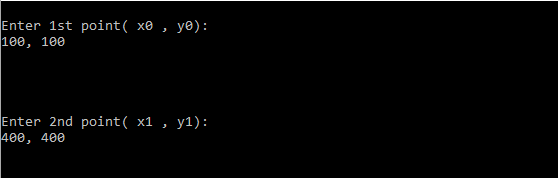
\includegraphics[height=2.0in]{input}
	\caption{Input two points to draw line}
\end{figure*}
\clearpage
\subsection{Output}
\begin{figure*}[!htb]
	\centering
	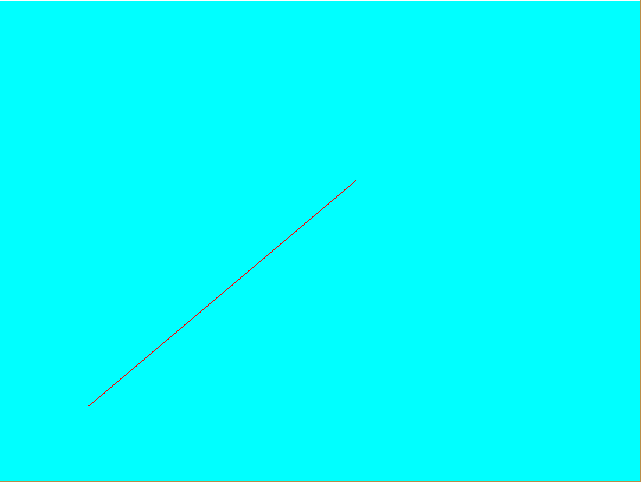
\includegraphics[height=3.0in,width=4in]{dda}
	\caption{Drawn line DDA algorithm}
\end{figure*}

\section{Discussion}
\begin{enumerate}[(i)]
	\item In this experiment we have learnt basic use of OpenGL.
	\item We have learnt how geometric line drawing is different in graphics line drawing.
	\item As DDA algorithm calculates steps and rounds the value the line pixels have some visible distortions.
	\item We have faced difficulties to run the program initially but eventually solved that adding windows special header file for OpenGL
\end{enumerate}


\chapter{Impelementaion of Bresenham Circle drawing Algorithm}
\section{Objective}
To draw circle from given center point and radius using Bresenham’s Circle drawing Algorithm.
\section{Used Tools}
\begin{itemize}
	\item OpenGL
	\item CodeBlocks IDE
\end{itemize}

\section{Description}
Drawing a circle on the screen is a little complex than drawing a line. There are two popular algorithms for generating a circle − Bresenham’s Algorithm and Midpoint Circle Algorithm.These algorithms are based on the idea of determining the subsequent points required to draw the circle.The equation of circle is-
$ X^2+Y^2=r^2 $, where r is radius.

We cannot display a continuous arc on the raster display. Instead, we have to choose the nearest pixel position to complete the arc.

From the following illustration, you can see that we have put the pixel at $(X, Y)$ location and now need to decide where to put the next pixel − at $N (X+1, Y)$ or at $S (X+1, Y-1) $.

This can be decided by the decision parameter d.
\begin{itemize}
	\item  If $d <= 0$, then $N(X+1, Y)$ is to be chosen as next pixel.
	\item If $d > 0$, then $S(X+1, Y-1)$ is to be chosen as the next pixel.
\end{itemize}

\section{Source Code}
\begin{lstlisting}
#include <windows.h>
#include <stdio.h>
#include <GL/glut.h>
#include <math.h>
int first=0;
int xi,yi,xf,yf;
void putpixel(int x,int y)
{
	glBegin(GL_POINTS);
	glVertex2i(x,y);
	glEnd();
	glFlush();
}
double round(double n)
{
	return (n >=0)?(int)(n+0.5):(int)(n-0.5);
}
void Bresenham_circle()
{
	int x=0,y=30,d=3-2*30;
	while(x <=y){
	//Here Transform each x,y coordinates by 250 pixels
	putpixel(250+x, 250+y);
	putpixel(250+y, 250+x);
	putpixel(250-x, 250+y);
	putpixel(250-x, 250-y);
	putpixel(250-y, 250+x);
	putpixel(250-y, 250-x);
	putpixel(250+y, 250-x);
	putpixel(250+x, 250-y);
	if(d< 0)
		d=d+(4*x)+6;
	else{
		d=d+(4*(x-y))+10;
		y--;
	}
	x++;
	}
}
void display()
{
	glClear (GL_COLOR_BUFFER_BIT);
	glColor3f (0.0, 0.0, 0.0);
	glPointSize(1.0);
	Bresenham_circle();
	glFlush();
}
void myinit()
{
	glClearColor(1.0, 1.0, 1.0, 0.0);
	glColor3f(0.0f, 0.0f, 0.0f);
	glPointSize(4.0);
	glMatrixMode(GL_PROJECTION);
	glLoadIdentity();
	gluOrtho2D(0.0, 640.0, 0.0, 480.0);
}
int main(int argc,char** argv)
{
	glutInit(&argc, argv);
	glutInitDisplayMode (GLUT_SINGLE | GLUT_RGB);
	glutInitWindowSize (640, 480);
	glutInitWindowPosition (100, 150);
	glutCreateWindow("Bresenham-Circle");
	glutDisplayFunc(display);
	myinit();
	glutMainLoop();
	return 0;
}
\end{lstlisting}
\clearpage
\section{Input \& Output}
\begin{figure*}[h]
	\centering
	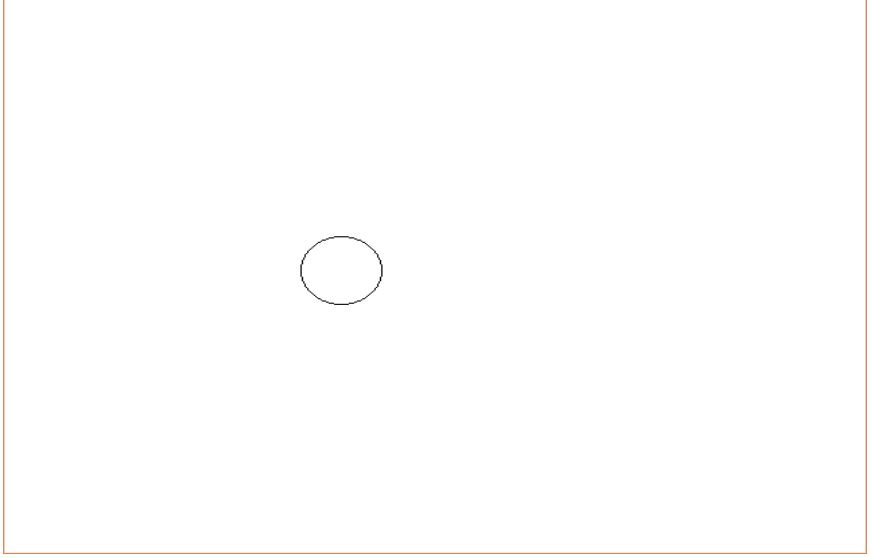
\includegraphics[height=3.0in,width=4.5in]{bres_circle_out}
	\caption{Output of Bresenham Circle Algorithm}
	
\end{figure*}
\section{Discussion}
\begin{enumerate}[(i)]
	\item In this experiment we have learnt about the circle in graphics remains symmetrical at 8 points.
	\item The circle we draw was initially broken as we took decision parameter equation wrong. It was solved debugging.
	\item In this program there is a deficiency that we didn't take user input for simplicity. So circle is fixed until edited in the code.
	\item The circle has some  distortions along perimeter because of the algorithm.
\end{enumerate}


\chapter{Impelementaion of Mid-Point Circle Algorithm}
\section{Objective}
To draw circle from given center point and radius using Midpoint Circle drawing Algorithm.
\section{Used Tools}
\begin{itemize}
	\item OpenGL
	\item CodeBlocks IDE
\end{itemize}

\section{Description}
We know the equation of circle is-
$ X^2+Y^2=r^2 $, where r is radius.
What we'd like to do is to use this discriminating function to maintain our trajectory of drawn pixels as close as possible to the desired circle. Luckily, we can start with a point on the circle, $(x_0, y_0 + r)$ (or $(0, r)$ in our adjusted coordinate system). As we move along in steps of x we note that the slope is less than zero and greater than negative one at points in the direction we're heading that are near our known point on a circle. Thus we need only to figure out at each step whether to step down in y or maintain y at each step.
\newline
We will compute points between x=0 and x=y and then draw the 8 matching points In that area, the slope of the curve is between 0 and -1
From each step/point $(x, y)$, the next one is either $(x+1, y)$ or $(x+1, y-1)$
We decide about which one by looking at the midpoint M.
\begin{figure*}[h]
	\centering
	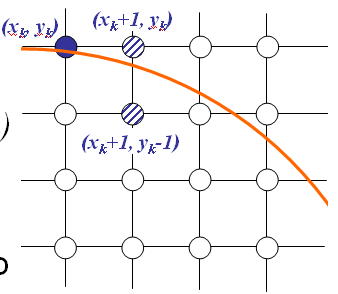
\includegraphics[height=3.0in]{b_circle1}
	\caption{Finding Midpoint}	
\end{figure*}

\begin{itemize}
	\item  M inside $(f<0) =>$ next point is E
	\item M outside $(f>0) =>$ next point is SE
\end{itemize}

\section{Algorithm}
\begin{enumerate}[(i)]
	\item Input radius r and circle center $(xc,yc)(xc,yc)$ and obtain the first point on the circumference of the circle centered on the origin as $(x0, y0) = (0, r)$
	\item Calculate the initial value of decision parameter as
	\begin{align*}	
	P_0 &= 5/4 – r\\
	f(x, y) &= x^2 + y^2 - r^2\\ &= 0\\
	f(x_i - 1/2 + e, y_i + 1)
	&= (x_i - \frac{1}{2} + e)^2 + (y_i + 1)^2 - r^2 \\
	&= (x_i- \frac{1}{2})^2 + (y_i + 1)^2 - r^2 + 2(xi - \frac{1}{2})e + e^2\\
	&= f(x_i - \frac{1}{2}, y_i + 1) + 2(x_i - \frac{1}{2})e + e^2 = 0\\
	\end{align*}
	Let,
	\begin{align*}
	d_i &= f(xi - \frac{1}{2}, y_i + 1) \\
	&= -2(x_i - \frac{1}{2})e - e^2 \\
	\end{align*}
	$\text{Thus, If}+ e < 0 +\text{then} d_i > 0 \text{so choose point}$
	\begin{align*}
	S &= (x_i - 1, y_i + 1)\\
	d_{i+1}    &= f(x_i - 1 - \frac{1}{2}, y_i + 1 + 1) \\
	&= ((x_i - \frac{1}{2}) - 1)^2 + ((y_i + 1) + 1)^2 - r^2\\
	&= d_i - 2(x_i - 1) + 2(y_i + 1) + 1\\
	&= d_i + 2(y_i + 1 - x_i + 1) + 1\\
	\end{align*}
	If $e >= 0$ then $d_i <= 0$ so choose point 
	\begin{align*}
	T &= (x_i, y_i + 1)\\
	d_i+1 &= f(x_i - \frac{1}{2}, y_i + 1 + 1)\\
	&= d_i + 2y_i+1 + 1
	\end{align*}	
	The initial value of $d_i$ is,
	\begin{align*}
	d_0 &= f(r - \frac{1}{2}, 0 + 1) \\
	&= (r - \frac{1}{2})2 + 12 - r^2\\
	&= \frac{5}{4} - r\\ \text{($1-r$ can be used if r is an integer)}
	\end{align*}
	\begin{lstlisting}			
	When point S = (x_i - 1, y_i + 1) is chosen then
	d_i+1 &= d_i + -2x_i+1 + 2y_i+1 + 1
	When point T = (x_i, y_i + 1) is chosen then
	d_i+1 = d_i + 2y_i+1 + 1
	\end{lstlisting}
	\item At each $X_K$ position starting at K=0, perform the following test 
	\newline If $(P_K < 0)$ then next point on circle (0,0) is $(X_{K+1},Y_K)$ and
	\begin{align*}
	PK+1 &= P_K + 2X_{K+1} + 1
	\end{align*}
	Else
	\begin{align*}
	P_{K+1} &= P_K + 2X_{K+1} + 1 – 2Y_{K+1}
	\end{align*}
	Where, 
	\begin{align*}
	2X_{K+1} &= 2X_{K+2} &\text{and} && 2Y_{K+1} &= 2Y_{K-2}
	\end{align*}
	\item Determine the symmetry points in other seven octants.
	\item Move each calculate pixel position $(X, Y)$ onto the circular path centered on $(X_C,Y_C)(X_C,Y_C)$ and plot the coordinate values.
	
	$X = X + X_C$,   $Y = Y + Y_C$
	\item Repeat step-(iii) through (v) until $X >= Y$.
\end{enumerate}

\section{Source Code}
\begin{lstlisting}
#include <windows.h>
#include <stdio.h>
#include <iostream>
#include <GL/glut.h>
#include <bits/stdc++.h>
int pntX1, pntY1, r;
void plot(int x, int y)
{
	glBegin(GL_POINTS);
	glVertex2i(x+pntX1, y+pntY1);
	glEnd();
}
void myInit (void)
{
	glClearColor(1.0, 1.0, 1.0, 0.0);
	glColor3f(0.0f, 0.0f, 0.0f);
	glPointSize(4.0);
	glMatrixMode(GL_PROJECTION);
	glLoadIdentity();
	gluOrtho2D(0.0, 640.0, 0.0, 480.0);
}
void midPointCircleAlgo()
{
	int x = 0;
	int y = r;
	float decision = 5/4 - r; //Po = 1 -r
	plot(x, y);
	while (y > x)
	{
	if (decision < 0)
		{
			x++;
			decision += 2*x+1; //Pk+1 = Pk + 2Xk+1 +1
		}
	else
	{
		y--;
		x++;
		decision += 2*(x-y)+1; //pk+1 = pk + 2xk+1 + 1 – 2yk+1
	}
	plot(x, y);
	plot(x, -y);
	plot(-x, y);
	plot(-x, -y);
	plot(y, x);
	plot(-y, x);
	plot(y, -x);
	plot(-y, -x);
}
}

void myDisplay(void)
{
	glClear (GL_COLOR_BUFFER_BIT);
	glColor3f (0.0, 0.0, 0.0);
	glPointSize(1.0);
	midPointCircleAlgo();
	glFlush ();
}

int main(int argc, char** argv)
{
	std::cout << "Enter the coordinates of the center:\n\n" << std::endl;
	std::cout << "X   : "; std::cin >> pntX1;
	std::cout << "\nY : "; std::cin >> pntY1;
	std::cout << "\nRadius? : "; std::cin >> r;
	glutInit(&argc, argv);
	glutInitDisplayMode (GLUT_SINGLE | GLUT_RGB);
	glutInitWindowSize (640, 480);
	glutInitWindowPosition (100, 150);
	glutCreateWindow ("MidPoint Circle Alogrithms");
	glutDisplayFunc(myDisplay);
	myInit ();
	glutMainLoop();

}

.
\end{lstlisting}

\section{Input \& Output}
\subsection{Input}

\begin{figure*}[!htb]
	\centering
	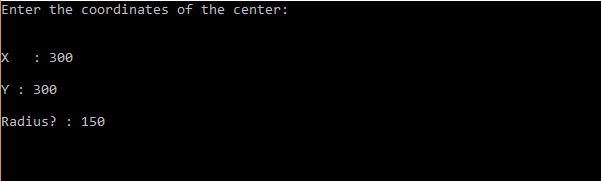
\includegraphics[height=1.5in]{midpoint_input}
	\caption{Input of Midpoint Circle Algorithm}
\end{figure*}

\subsection{Output}
\begin{figure*}[!htb]
	\centering
	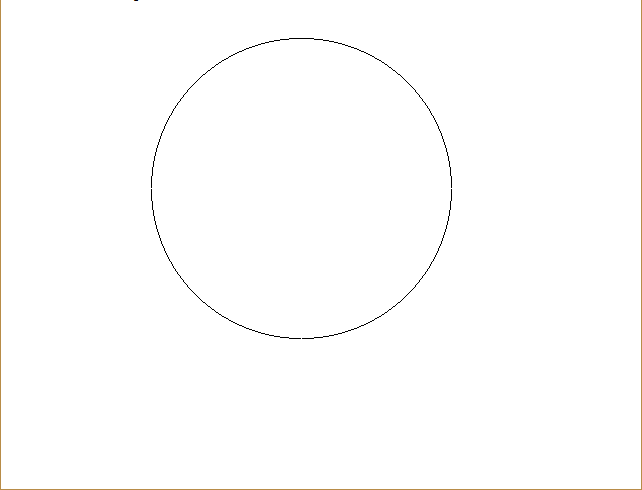
\includegraphics[height=2.0in]{midpoint_circle_out}
	\caption{Output of Midpoint Circle Algorithm}
\end{figure*}

\section{Discussion}
\begin{enumerate}[(i)]
	\item In this experiment we have learnt about the circle in graphics remains symmetrical at 8 points.
	\item In this program there is a deficiency that we didn't take user input for simplicity. So circle is fixed until edited in the code.
	\item The circle has some  distortions along perimeter because of the algorithm.
\end{enumerate}

\chapter{Scan convert an ellipse using midpoint ellipse algorithm}
\section{Objective}
To scan convert an ellipse using Midpoint ellipse algorithm.
\section{Used Tools}
\begin{itemize}
	\item OpenGL
	\item CodeBlocks IDE
\end{itemize}

\section{Description}
Midpoint ellipse algorithm is a method for drawing ellipses in computer graphics. Let us consider one quarter of an ellipse. The curve is divided into two regions. In region I, the slope on the curve is greater than –1 while in region II less than –1. Consider the general equation of an ellipse, 
$b^2x^2 + a^2y^2 - a^2b^2 = 0$
where a is the horizontal radius and b is the vertical radius, we can define an function f(x,y) by which the error due to a prediction coordinate (x,y) can be obtained. The appropriate pixels can be selected according to the error so that the required ellipse is formed. The error can be confined within half a pixel.

\begin{figure*}[h]
	\centering
	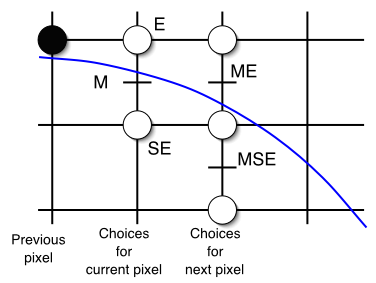
\includegraphics[height=2.0in,width=2.5in]{midPoint}
	\caption{Finding Midpoint}	
\end{figure*}

Set $f(x,y) = b^2x^2 + a^2y^2 – a^2b^2$
\newline In region $I (dy/dx > –1)$,
$(x_{k+1}, y_{k\frac{-1}{2}})$
\newline
x is always incremented in each step, i.e. $x_{k+1} = x_{k + 1}$. $y_{k+1} = y_k$ if E is selected, or $y_{k+1} = y_k – 1$ if SE is selected. In order to make decision between S and SE, a prediction $(x_{k+1}, y_{k\frac{-1}{2}})$ is set at the middle between the two candidate pixels.

\section{Source Code}
\begin{lstlisting}
#include <windows.h>
#include<gl/glut.h>
#include<gl/glu.h>
#include<gl/gl.h>
#include<iostream>

using namespace std;
int xc=0,yc=0,a=60,b=30;

void display(){
	float asq=a*a;
	float bsq=b*b;
	float x=0,y=b,p;
	float px=0,py=2*asq*y;
	glClear(GL_COLOR_BUFFER_BIT);
	glPointSize(1);
	glBegin(GL_POINTS);
	glVertex2i(xc+x,yc+y);
	glVertex2i(-(xc+x),-(yc+y));
	cout<<xc+x<<" "<<yc+y<<endl;
	
	//region 1
	p=bsq-(asq-b)+(0.25*asq);
	while(px<py){
		x++;
		px=px+2*bsq;
		if(p<0) p=p+bsq+px;
		else{
			y--;
			py=py-2*asq;
			p=p+bsq+px-py;
		}
		glVertex2i(xc+x,yc+y);
		glVertex2i(xc+x,-(yc+y));
		glVertex2i(-(xc+x),yc+y);
		glVertex2i(-(xc+x),-(yc+y));
		cout<<xc+x<<" "<<yc+y<<endl;
	}
	
	//region 2
	p=bsq*(x+0.5)*(x+0.5) + asq*(y-1)*(y-1) -asq*bsq;
	while(y>0){
		y--;
		py=py-2*asq;
		if(p>0){
			p=p+asq-py;
		}else{
			x++;
			px=px+2*bsq;
			p=p+asq-py+px;
		}
	
	glVertex2i(xc+x,yc+y);
	glVertex2i(xc+x,-(yc+y));
	glVertex2i(-(xc+x),yc+y);
	glVertex2i(-(xc+x),-(yc+y));
	cout<<xc+x<<" "<<yc+y<<endl;
	}
	glEnd();
	glFlush();
}
void init(){
	glMatrixMode(GL_PROJECTION);
	glLoadIdentity();
	gluOrtho2D(-100,100,-100,100);
}
int main(int argc, char** argv){
	glutInit(&argc, argv);
	glutInitDisplayMode (GLUT_SINGLE | GLUT_RGB);
	glutInitWindowSize (500, 500);
	glutInitWindowPosition (100, 100);
	glutCreateWindow ("Mid Point Ellipse Algorithm ");
	init ();
	glutDisplayFunc(display);
	glutMainLoop();
	return 0;
}

\end{lstlisting}
\section{Input \& Output}
\begin{figure*}[ht!]
	\centering
	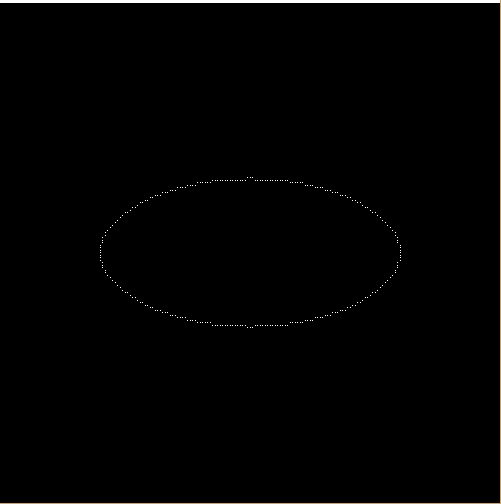
\includegraphics[height=3.0in,width=3.5in]{ellipse}
	\caption{Output of Midpoint Ellipse Algorithm}
\end{figure*}
\section{Discussion}
\begin{enumerate}[(i)]
	\item This method is modified from Bresenham’s algorithm.
	\item The advantage of this modified method is that only addition operations are required in the program loops. This leads to simple and fast implementation in all processors.
	\item In this program there is a deficiency that we didn't take user input for simplicity. So circle is fixed until edited in the code.
	\item The ellipse has some  distortions along perimeter because of the algorithm.
\end{enumerate}




\chapter{Impelementation of Boundary fill algorithm}
\section{Objective}
To fill a given shape using boundary fill algorithm.
\section{Used Tools}
\begin{itemize}
	\item OpenGL
	\item CodeBlocks IDE
\end{itemize}

\section{Description}
This algorithm picks a point inside an figure and starts to fill until it reaches the boundary of the figure. The color of the boundary and the color that we fill should be different for this algorithm to work.In this algorithm, we assume that color of the boundary is same for the entire figure. The boundary fill algorithm can be implemented by 4-connected pixels or 8-connected pixels. Filling continues until a boundary color is encountered. The problem with four fill is some area is left unfilled. This leads to the  Eight-connected fill algorithm where we test all eight adjacent pixels.

\section{Algorithm}
\begin{lstlisting}
Procedure Four_Fill (x, y, fill_col, bound_col: integer);
var
curr_color: integer;
begin
curr_color := inquire_color(x, y)
if (curr_color <> bound color) and (curr_color <> fill_col) then
begin
set_pixel(x, y, fill_col)
Four_Fill (x+1, y, fill_col, bound_col);
Four_Fill (x-1, y, fill_col, bound_col);
Four_Fill (x, y+1, fill_col, bound_col);
Four_Fill( x, y-1, fill_col, bound_col);
end;
`
\end{lstlisting}

\section{Source Code}
\begin{lstlisting}
#include<windows.h>
#include<GL/glut.h>
#include<stdio.h>
#include<stdlib.h>
#include<time.h>
#include<math.h>

struct Point {
	GLint x;
	GLint y;
};

struct Color {
	GLfloat r;
	GLfloat g;
	GLfloat b;
};

void init() {
	glClearColor(1.0, 1.0, 1.0, 0.0);
	glColor3f(0.0, 0.0, 0.0);
	glPointSize(1.0);
	glMatrixMode(GL_PROJECTION);
	glLoadIdentity();
	gluOrtho2D(0, 640, 0, 480);
}

Color getPixelColor(GLint x, GLint y) {
	Color color;
	glReadPixels(x, y, 1, 1, GL_RGB, GL_FLOAT, &color);
	return color;
}

void setPixelColor(GLint x, GLint y, Color color) {
	glColor3f(color.r, color.g, color.b);
	glBegin(GL_POINTS);
	glVertex2i(x, y);
	glEnd();
	glFlush();

}

void BoundaryFill(int x, int y, Color fillColor, Color boundaryColor) {
	Color currentColor = getPixelColor(x, y);
	if(currentColor.r != boundaryColor.r && currentColor.g != boundaryColor.g &&
	 currentColor.b != boundaryColor.b) {
	setPixelColor(x, y, fillColor);
	BoundaryFill(x+1, y, fillColor, boundaryColor);
	BoundaryFill(x-1, y, fillColor, boundaryColor);
	BoundaryFill(x, y+1, fillColor, boundaryColor);
	BoundaryFill(x, y-1, fillColor, boundaryColor);
}
}

void onMouseClick(int button, int state, int x, int y){
	Color fillColor = {1.0f, 1.0f, 0.0f};		// red color will be filled
	Color boundaryColor = {0.0f, 0.0f, 0.0f}; // black- boundary
	Point p = {321, 241}; // a point inside the circle
	BoundaryFill(p.x, p.y, fillColor, boundaryColor);
}

void draw_circle(Point pC, GLfloat radius) {
	GLfloat step = 1/radius;
	GLfloat x, y;
	for(GLfloat theta = 0; theta <= 360; theta += step) {
		x = pC.x + (radius * cos(theta));
		y = pC.y + (radius * sin(theta));
		glVertex2i(x, y);
	}
}

void display(void) {
	Point pt = {320, 240};
	GLfloat radius = 70;
	glClear(GL_COLOR_BUFFER_BIT);
	glBegin(GL_POINTS);
	draw_circle(pt, radius);
	glEnd();
	glFlush();
}

int main(int argc, char** argv){
	glutInit(&argc, argv);
	glutInitDisplayMode(GLUT_SINGLE|GLUT_RGB);
	glutInitWindowSize(640, 480);
	glutInitWindowPosition(200, 200);
	glutCreateWindow("Boundary Fill Algorithm");
	init();
	glutDisplayFunc(display);
	glutMouseFunc(onMouseClick);
	glutMainLoop();
	return 0;
}

\end{lstlisting}
\section{Input \& Output}
\begin{figure*}[ht!]
	\centering
	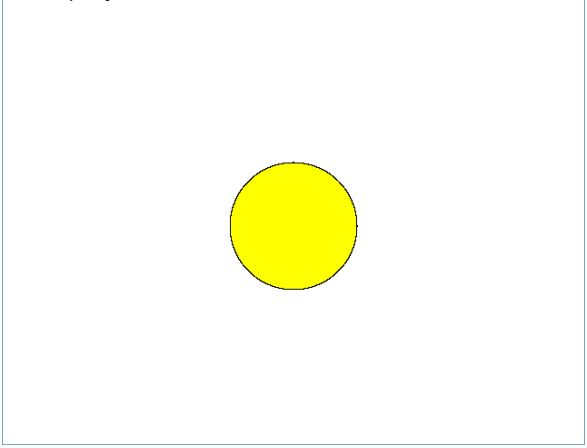
\includegraphics[height=2.3in]{boundery_output}
	\caption{Output after Boundary fill of a circle}
\end{figure*}

\section{Discussion}
\begin{enumerate}[(i)]
	\item We have used four fill algorithm here which is inefficient but serves our objective
	\item We faced some problem while running the code because of GLUT integration problem but we solved that by debugging.
\end{enumerate}


\chapter{Impelementation of Flood fill algorithm}
\section{Objective}
To fill a given shape using flood fill algorithm.
\section{Used Tools}
\begin{itemize}
	\item OpenGL
	\item CodeBlocks IDE
\end{itemize}


\section{Description}
Sometimes we come across a figure where we want to fill the area and its boundary of the figure with different colors. We can paint such figure with a specific color instead of searching for particular boundary color as in boundary filling algorithm. Instead of relying on the boundary of the figure, it relies on the fill color. In other words, it replaces the interior color of the figure with the fill color. When no more pixels of the original interior color exist, the algorithm is completed.

\section{Algorithm}
\begin{lstlisting}

void floodFill4(int x, int y, int newColor, int oldColor)
{
if(x >= 0 && x < w && y >= 0 && y < h && screenBuffer[y][x][y] == oldColor && screenBuffer[x] != newColor)
{
screenBuffer[y][x] = newColor; //set color before starting recursion

floodFill4(x + 1, y    , newColor, oldColor);
floodFill4(x - 1, y    , newColor, oldColor);
floodFill4(x    , y + 1, newColor, oldColor);
floodFill4(x    , y - 1, newColor, oldColor);
}
}
\end{lstlisting}

\section{Source Code}
\begin{lstlisting}
#include<windows.h>
#include<GL/glut.h>
#include<stdio.h>
#include<stdlib.h>
#include<time.h>
#include<math.h>
// grouped list of point variables
struct Point {
	GLint x;
	GLint y;
};
// grouped list of point variables
struct Color {
	GLfloat r;
	GLfloat g;
	GLfloat b;
};
void init() {
	glClearColor(0.0, 1.0, 0.0, 0.0); // specify clear values for the color buffers
	glColor3f(0.0, 0.0, 0.0);         //Sets the current color.
	glPointSize(1.0);
	glMatrixMode(GL_PROJECTION); // specify which matrix is the current matrix.
	//subsequent matrix operations to the projection matrix stack.
	glLoadIdentity();      // replace the current matrix with the identity matrix
	gluOrtho2D(0, 640, 0, 480);  //define a 2D orthographic projection matrix
}
Color getPixelColor(GLint x, GLint y) {
	Color color;
	glReadPixels(x, y, 1, 1, GL_RGB, GL_FLOAT, &color);  
	//read a block of pixels from the frame buffer
	return color;
}
void setPixelColor(GLint x, GLint y, Color color) {
	glColor3f(color.r, color.g, color.b); //Sets the current color.
	glBegin(GL_POINTS); 
	glVertex2i(x, y);//Specifies a vertex.
	glEnd();
	glFlush(); //force execution of GL commands in finite time
}
void floodFill(GLint x, GLint y, Color oldColor, Color newColor) {
	Color color;
	color = getPixelColor(x, y);
	
	if(color.r == oldColor.r && color.g == oldColor.g && color.b == oldColor.b)
	{
		setPixelColor(x, y, newColor);
		floodFill(x+1, y, oldColor, newColor);
		floodFill(x, y+1, oldColor, newColor);
		floodFill(x-1, y, oldColor, newColor);
		floodFill(x, y-1, oldColor, newColor);
	}
	return;
}
void onMouseClick(int button, int state, int x, int y)
{
	Color newColor = {1.0f, 0.0f, 0.0f};
	Color oldColor = {0.0f, 1.0f, 0.0f};
	
	floodFill(320, 240, oldColor, newColor);
}
void draw_circle(Point pC, GLfloat radius) {
	GLfloat step = 1/radius;
	GLfloat x, y;
	
	for(GLfloat theta = 0; theta <= 360; theta += step) {
		x = pC.x + (radius * cos(theta));      //calculate the x component
		y = pC.y + (radius * sin(theta));      //calculate the x component
		glVertex2i(x, y);                   //Specifies a vertex.
	}
}
void display(void) {
	Point pt = {320, 240};
	GLfloat radius = 70;
	glClear(GL_COLOR_BUFFER_BIT); // clear buffers to preset values
	//buffers currently enabled for color writing 
	//GL_DEPTH_BUFFER_BIT, GL_STENCIL_BUFFER_BIT
	glBegin(GL_POINTS);
	draw_circle(pt, radius);
	glEnd();
	glFlush();
}
int main(int argc, char** argv)
{
	glutInit(&argc, argv); //initialize the GLUT library.
	glutInitDisplayMode(GLUT_SINGLE|GLUT_RGB); // sets the initial display mode. 
	//GLUT_SINGLE -Bit mask to select a single buffered window.
	//GLUT_RGBA-Bit mask to select an RGBA mode window
	glutInitWindowSize(640, 480);
	glutInitWindowPosition(200, 200);//window position and size respectively
	glutCreateWindow("Flood Fill Algorithm");
	init();
	glutDisplayFunc(display); //display callback for the current window
	glutMouseFunc(onMouseClick);
	glutMainLoop();          //enters the GLUT event processing loop.
	return 0;
}

\end{lstlisting}
\clearpage
\section{Input \& Output}
\begin{figure*}[ht!]
	\centering
	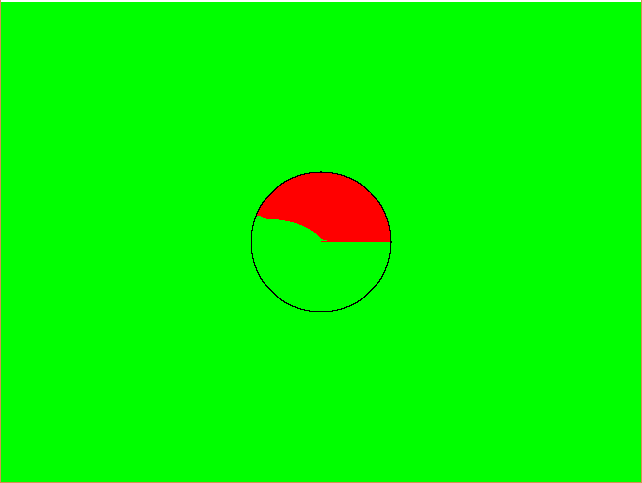
\includegraphics[height=3.0in]{flood_out}
	\caption{Output Started Flooding area}
\end{figure*}
\begin{figure*}[ht!]
	\centering
	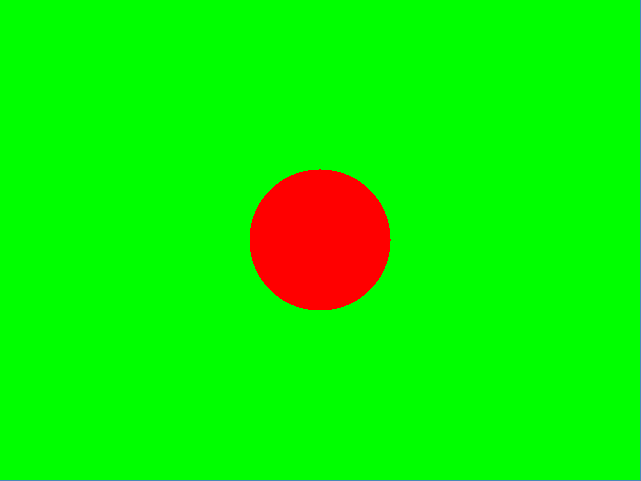
\includegraphics[height=3.0in]{flood_out1}
	\caption{Output after Boundary fill of a circle}
\end{figure*}


\section{Discussion}
\begin{enumerate}[(i)]
	\item We have learnt how we can fill an area without finding boundary color first.
	\item Sometimes because of heavy recursion processor becomes slow and fills the area slowly. 
\end{enumerate}




\chapter{Drawing C curve}
\section{Objective}
To draw C curve with different iteration.
\section{Used Tools}
\begin{itemize}
	\item Java
	\item Java Compiler
\end{itemize}

\section{Description}
Fractals are very complex pictures generated by a computer from a single formula. They are created using iterations. This means one formula is repeated with slightly different values over and over again, taking into account the results from the previous iteration. An isosceles triangle with angles of 45°, 90° and 45° is built using this line as its hypotenuse. The original line is then replaced by the other two sides of this triangle. At the second stage, the two new lines each form the base for another right-angled isosceles triangle, and are replaced by the other two sides of their respective triangle. So, after two stages, the curve takes the appearance of three sides of a rectangle with the same length as the original line, but only half as wide. At each subsequent stage, each straight line segment in the curve is replaced by the other two sides of a right-angled isosceles triangle built on it. After n stages the curve consists of 2n line segments, each of which is smaller than the original line by a factor of $2\frac{n}{2}$.

\section{Algorithm}
\begin{lstlisting}
L-system can be described as follows:

Variables:	F
Constants:	+ −
Start:	F
Rules:	F → +F−−F+
.
\end{lstlisting}

\section{Source Code}
\begin{lstlisting}
import java.awt.Color;
import java.awt.Graphics;
import java.awt.Graphics2D;
import javax.swing.JFrame;
import javax.swing.JPanel;
import java.util.concurrent.ThreadLocalRandom;

public class C_curve extends JPanel {

public float x, y, len, alpha_angle;
public int iteration_n;

public void paint(Graphics g) {
	Graphics2D g2d = (Graphics2D) g;
	c_curve(x, y, len, alpha_angle, iteration_n, g2d);
}

public void c_curve(double x, double y, double len, double alpha_angle, int 
iteration_n, Graphics2D g) {
	double fx = x; 
	double fy = y;
	double length = len;
	double alpha = alpha_angle;
	int it_n = iteration_n;
	if (it_n > 0) {
	length = (length / Math.sqrt(2));
	c_curve(fx, fy, length, (alpha + 45), (it_n - 1), g); // Recursive Call
	fx = (fx + (length * Math.cos(Math.toRadians(alpha + 45))));
	fy = (fy + (length * Math.sin(Math.toRadians(alpha + 45))));
	c_curve(fx, fy, length, (alpha - 45), (it_n - 1), g); // Recursive Call
	} else {
	Color[] A = {Color.RED, Color.ORANGE, Color.BLUE, Color.DARK_GRAY};
	g.drawLine((int) fx, (int) fy, (int) (fx + (length *
	 Math.cos(Math.toRadians(alpha)))), (int) (fy + (length *
	  Math.sin(Math.toRadians(alpha)))));
}
}

public static void main(String[] args) {
	C_curve points = new C_curve();
	points.x = 200; // Stating x value
	points.y = 100; // Stating y value
	points.len = 150; // Stating length value
	points.alpha_angle = 90; // Stating angle value
	points.iteration_n = 11; // Stating iteration value
	
	JFrame frame = new JFrame("C Curve 1204028");
	frame.setDefaultCloseOperation(JFrame.EXIT_ON_CLOSE);
	frame.add(points);
	frame.setSize(500, 500);
	frame.setLocationRelativeTo(null);
	frame.setVisible(true);

}
}

\end{lstlisting}
\clearpage
\section{Input \& Output}
\begin{figure*}[ht!]
	\centering
	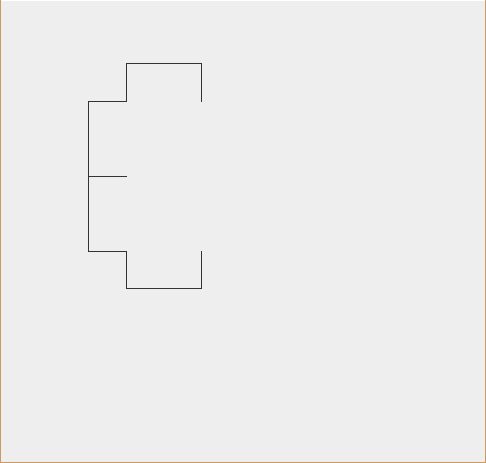
\includegraphics[height=3.0in,width=3.5in]{c_curve_4}
	\caption{C Curve after 4 iteration}
\end{figure*}


\section{Discussion}
\begin{enumerate}[(i)]
	\item In this curve every iteration isosceles triangle forms. 
	\item We have used java to complete this experiment as java also provides graphical interface 
	\item We have got output using different iteration and it looks like C letter. 
\end{enumerate}




\chapter{Drawing Koch curve}
\section{Objective}
To draw Koch curve with different iteration.
\section{Used Tools}
\begin{itemize}
	\item OpenGL
	\item CodeBlocks IDE
\end{itemize}

\section{Description}
The Koch snowflake (also known as the Koch curve, Koch star, or Koch island) is a mathematical curve. The progression for the area of the snowflake converges to 
$\frac{8}{5}$ times the area of the original triangle, while the progression for the snowflake's perimeter diverges to infinity. Consequently, the snowflake has a finite area bounded by an infinitely long line. The Koch snowflake can be constructed by starting with an equilateral triangle, then recursively altering each line segment. After one iteration of this process, the resulting shape is the outline of a hexagram. The Koch snowflake is the limit approached as the above steps are followed over and over again. The Koch curve originally described by Helge von Koch is constructed with only one of the three sides of the original triangle. In other words, three Koch curves make a Koch snowflake.

\section{Algorithm}

\begin{enumerate}[(i)]
	\item divide the line segment into three segments of equal length.
	\item draw an equilateral triangle that has the middle segment from step (i) as its base and points outward.
	\item remove the line segment that is the base of the triangle from step (ii).
\end{enumerate}

\section{Source Code}
\begin{lstlisting}
#include <windows.h>
#include <GL/glut.h>
#include <math.h>
GLfloat currentX=-0.7,currentY=0.5;

void drawkoch(GLfloat degree,GLfloat len,GLint iter) {
	GLdouble degreeRad = 0.0174533 * degree;
	GLfloat newX = currentX + len * cos(degreeRad);
	GLfloat newY = currentY + len * sin(degreeRad);
	if (iter==0) {
		glVertex2f(currentX, currentY);
		glVertex2f(newX, newY);
		currentX = newX;
		currentY = newY;
	}else {
		iter--;
		//draw the four parts of the side _/\_
		drawkoch(degree, len, iter);
		degree += 60.0;
		drawkoch(degree, len, iter);
		degree -= 120.0;
		drawkoch(degree, len, iter);
		degree += 60.0;
		drawkoch(degree, len, iter);
	}
}
void mydisplay(){
	glClear( GL_COLOR_BUFFER_BIT );
	glBegin(GL_LINES);
	glColor3f(1.0, 1.0, 0.0); // yollow
	//call drawkoch 3 times, one for each side of the triangle, 
	//changing direction each time
	drawkoch(0.0,0.001,6);
	drawkoch(-120.0, 0.001, 6);
	drawkoch(120.0,0.001,6);
	glEnd();
	glFlush();
}
int main(int argc, char** argv){
	glutInit(&argc,argv);
	glutInitDisplayMode(GLUT_SINGLE|GLUT_RGB);
	glutInitWindowSize(500,500);
	glutInitWindowPosition(0,0);
	glutCreateWindow("Koch Curve 1204028");
	glutDisplayFunc(mydisplay);
	glutMainLoop();
}

\end{lstlisting}
\clearpage
\section{Input \& Output}
\begin{figure*}[ht!]
	\centering
	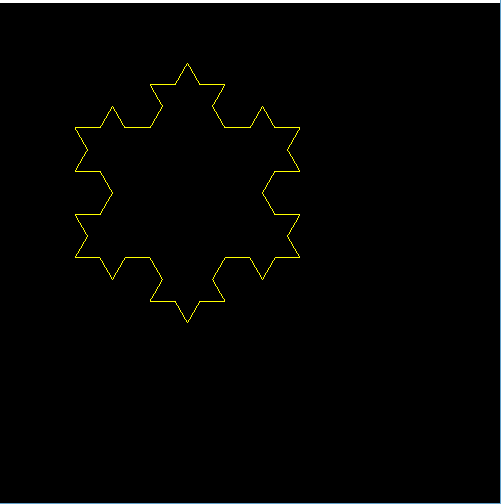
\includegraphics[height=3.0in,width=3.5in]{koch_2}
	\caption{Koch Curve after 2 iteration around a triangle}
\end{figure*}


\section{Discussion}
\begin{enumerate}[(i)]
	\item In this curve every iteration equilateral triangle forms. 
	\item Equlateral triangle has 60 degree angles but we have taken 120 triangle because if we turn clock wise from the line it generates 180-60=120 degree angle.
	\item We have drawn koch curve in a triangles each side that's why it looks like a snowflake.
\end{enumerate}

\chapter{Line clipping using Cohen-Sutherland line clipping algorithm}
\section{Objective}
Clip different lines using cohen-sutherland line clipping algorithm.
\section{Used Tools}
\begin{itemize}
	\item OpenGL
	\item CodeBlocks IDE
\end{itemize}

\section{Description}
This algorithm uses the clipping window as shown in the following figure. The minimum coordinate for the clipping region is (XWmin,YWmin)(XWmin,YWmin) and the maximum coordinate for the clipping region is (XWmax,YWmax)(XWmax,YWmax).
\newline
\begin{figure*}[!htb]
	\centering
	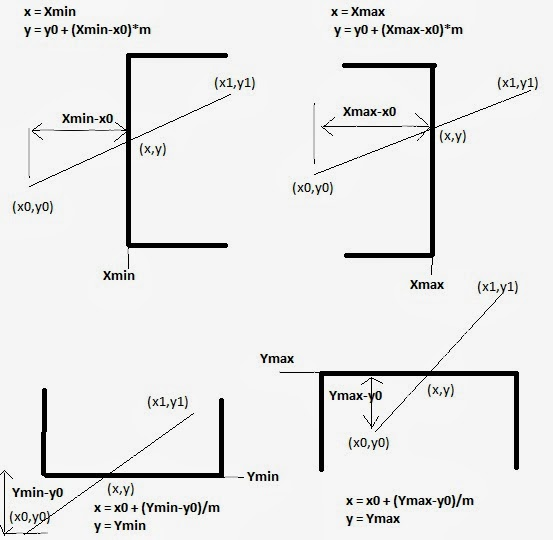
\includegraphics[height=3.5in,width=4in]{blogpic}
	\caption{Cohen Suderland Line Clip Equations}
\end{figure*}

We will use 4-bits to divide the entire region. These 4 bits represent the Top, Bottom, Right, and Left of the region as shown in the following figure. Here, the TOP and LEFT bit is set to 1 because it is the TOP-LEFT corner.
\begin{figure*}[!htb]
	\centering
	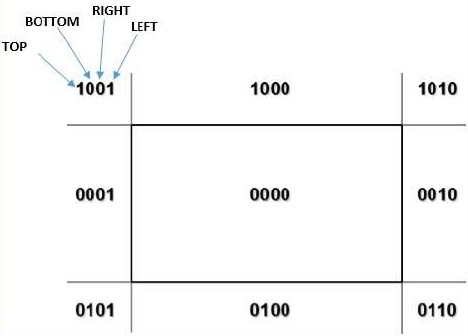
\includegraphics[height=2.0in]{reg_code}
	\caption{Region Codes}
\end{figure*}


There are 3 possibilities for the line −
\begin{enumerate}[(i)]
	\item Line can be completely inside the window (This line should be accepted).
	
	\item Line can be completely outside of the window (This line will be completely removed from the region).
	
	\item Line can be partially inside the window (We will find intersection point and draw only that portion of line that is inside region).
\end{enumerate}
\section{Algorithm}

\begin{enumerate}[(i)]
	\item Assign a region code for each endpoints.
	\item If both endpoints have a region code 0000 then accept this line.
	\item Else, perform the logical AND operation for both region codes.
	\begin{enumerate}[1]
		\item f the result is not 0000, then reject the line.
		\item Else we need clipping.
		\begin{enumerate}[I]
			\item Choose an endpoint of the line that is outside the window.
			\item Find the intersection point at the window boundary (base on region code).
			\item Replace endpoint with the intersection point and update the region code.
			\item Repeat step 2 until we find a clipped line either trivially accepted or trivially rejected.
			
		\end{enumerate}
	\end{enumerate}
	\item Repeat step (i) for other lines.
\end{enumerate}


\section{Source Code}
\begin{lstlisting}
#include<windows.h>
#include<stdio.h>
#include<GL/glut.h>
#define outcode int
double xmin=50,ymin=50,xmax=100,ymax=100;// Windows boundaries
double xvmin=200,yvmin =200, xvmax=300,yvmax=300; // Viewport boundaries
const int RIGHT= 8; // bit codes for the right
const int LEFT =2;  //bit codes for the left
const int TOP=4;    // bit codes for the top
const int BOTTOM=1; //bit codes for the bottom
outcode ComputeOutCode(double x,double y); // used to compute bit codes of a point
// Cohen -Sutherland clipping algorithm clips a line from
// p0=(x0,y0)  to p1 =(x1,y1) against a rectangle with.
// diagonal from (xmin,ymin)to (xmax,ymax)
void CohenSutherlandLineClipAnddraw(double x0,double y0,double x1,double y1){
	// OutCodes for P0 ,P1 and Whatever point(among P0 & P1) lies outside the
	// clip rectangle
	outcode outcode0,outcode1,outcodeOut;
	int accept =0,done =0;// These are two bits to indicate trivial accept and/or
	// done with clipping
	//compute outcodes
	outcode0= ComputeOutCode(x0,y0);
	outcode1= ComputeOutCode(x1,y1);
	do{
	if(!(outcode0|outcode1)) // logical or is 0 trivially accept and exit{ accept=1;
	done=1;
	}else
	if(outcode0 & outcode1)  // logical and is 0 trivially reject and exit
	done=1;
	else{
	//failed both tests , so calculate the line segment clip;
	// from an outside point to an intersection with clip edge
	double x,y;
	// at least one endpoint is outside the clip rectangle ; pick it.
	outcodeOut= outcode0?outcode0:outcode1;
	//now find the intersection point ; slope m= (y1-y0)/(x1-x0)
	// use formula
	// y=y0+slope*(x-x0), //either x is xmin or xmax
	// x=x0+(1/slope)*(y-y0) // y is ymin or ymax
	
	if(outcodeOut & TOP) //point is above the clip rectangle{
	x= x0+(x1-x0)*(ymax-y0)/(y1-y0);
	y=ymax;
	}else if(outcodeOut & BOTTOM) //point is below the clip rectangle{
	x= x0+(x1-x0)*(ymin-y0)/(y1-y0);
	y=ymin;
	}else if(outcodeOut & RIGHT) //point is to the right of clip rectangle{
	y= y0+(y1-y0)*(xmax-x0)/(x1-x0);
	x=xmax;
	}else                   //point is to the left of the clip rectangle{
	y= y0+(y1-y0)*(xmin-x0)/(x1-x0);
	x=xmin;
	}
	// now we move outside point to intersection point to clip
	// and get ready for next pass.
	if(outcodeOut == outcode0) // If the outside point was p0 update x0,y0 to x,y{ 	x0=x;                           // so x,y become the new x0,y0
		y0=y;
		outcode0 = ComputeOutCode(x0,y0);
		//compute outcode of new endpoint
	}else  // If the outside point was p1 update x1,y1 to x,y{     // so x,y becomes the new x1,y1
		x1=x;
		y1=y;
		outcode1 = ComputeOutCode(x1,y1);
		// compute outcode of new endpoint
	}
	}
	}while(!done);
	if(accept) //If line was trivial reject no need to draw viewport{
		// window to viewport mapping
		double sx=(xvmax-xvmin)/(xmax-xmin);// scale parameter in x direction
		double sy=(yvmax-yvmin)/(ymax-ymin);// scale parameter in y direction
		double vx0 = xvmin+(x0-xmin)*sx;
		double vy0 = yvmin+(y0-ymin)*sy;
		double vx1 = xvmin+(x1-xmin)*sx;
		double vy1 = yvmin+(y1-ymin)*sy;
		//draw a red color viewport
		glColor3f(1.0,0.0,0.0);
		glBegin(GL_LINE_LOOP);
		glVertex2f(xvmin,yvmin);
		glVertex2f(xvmax,yvmin);
		glVertex2f(xvmax,yvmax);
		glVertex2f(xvmin,yvmax);
		glEnd();
		glColor3f(0.0,1.0,0.0);
		glBegin(GL_LINES);
		glVertex2d(vx0,vy0);
		glVertex2d(vx1,vy1);
		glEnd();
	}
}
// compute the bit code for a point (x,y) using the clip rectangle
// bounded diagonally by (xmin,ymin) and (xmax,ymax)
outcode ComputeOutCode(double x,double y){
	outcode code =0;
	if(y>ymax)   //above the clip window
	code |=TOP;
	if(y<ymin)   //below the clip window
	code |=BOTTOM;
	if(x>xmax)        //to the right of the clip window
	code |=RIGHT;
	if(x<xmin)  //to the left of the clip window
	code |=LEFT;
	return code;
}
void display(){
	double x0=120,y0=10,x1=40,y1=130;
	glClear(GL_COLOR_BUFFER_BIT);
	glColor3f(0.0,1.0,0.0); // draw red color lines
	glBegin(GL_LINES);
	glVertex2d(x0,y0);
	glVertex2d(x1,y1);
	glVertex2d(60,20);
	glVertex2d(80,120);
	glEnd();
	glColor3f(0.0,0.0,1.0); // draw a blue colored window
	glBegin(GL_LINE_LOOP);
	glVertex2f(xmin,ymin);
	glVertex2f(xmax,ymin);
	glVertex2f(xmax,ymax);
	glVertex2f(xmin,ymax);
	glEnd();
	CohenSutherlandLineClipAnddraw(x0,y0,x1,y1);
	CohenSutherlandLineClipAnddraw(60,20,80,120);
	glFlush();
}
void myinit(){
	glClearColor(0.0,0.0,0.0,0.0);
	glColor3f(1.0,0.0,0.0);
	glPointSize(1.0);
	glMatrixMode(GL_PROJECTION);
	glLoadIdentity();
	gluOrtho2D(0.0,499.0,0.0,499.0);
}
int main(int argc, char** argv)
{
	glutInit(&argc,argv);
	glutInitDisplayMode(GLUT_SINGLE|GLUT_RGB);
	glClearColor(1.0f, 1.0f, 1.0f, 0.0f);
	glutInitWindowSize(800,600);
	glutInitWindowPosition(0,0);
	glutCreateWindow("Cohen Sutherland line clipping algorithm -1204028");
	glutDisplayFunc(display);
	myinit();
	glutMainLoop();
	return 0;
}
.

\end{lstlisting}

\section{Input \& Output}
\begin{figure*}[h!]
	\centering
	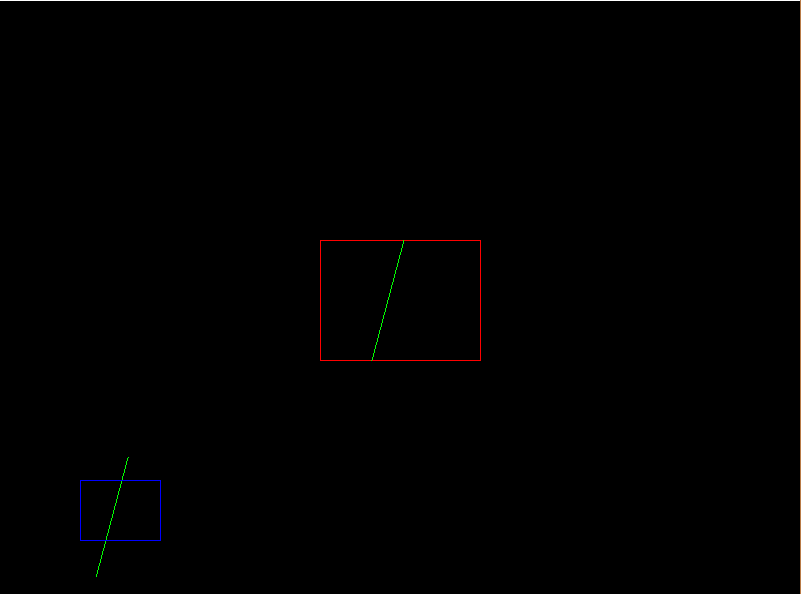
\includegraphics[height=3.0in, width=5in]{lineclip_1}
	\caption{Line clip 1}
\end{figure*}
\section{Discussion}
\begin{enumerate}[(i)]
	\item Line clip using cohen suderland algorithm was easy to understand but coding was difficult because of its conditions.
	\item We have drawn and clipped a fixed line and a changable line for understanding first.
	\item We didn't take user input of the lines points for simplicity.
\end{enumerate}




\chapter{Polygon clipping using Sutherland-\newline Hodgeman polygon clipping algorithm}
\section{Objective}
Clip polygon from a given window using Sutherland-Hodgeman algorithm
\section{Used Tools}
\begin{itemize}
	\item OpenGL
	\item CodeBlocks IDE
\end{itemize}

\section{Description}
The algorithm begins with an input list of all vertices in the subject polygon. Next, one side of the clip polygon is extended infinitely in both directions, and the path of the subject polygon is traversed. Vertices from the input list are inserted into an output list if they lie on the visible side of the extended clip polygon line, and new vertices are added to the output list where the subject polygon path crosses the extended clip polygon line. This process is repeated iteratively for each clip polygon side, using the output list from one stage as the input list for the next. Once all sides of the clip polygon have been processed, the final generated list of vertices defines a new single polygon that is entirely visible. Note that if the subject polygon was concave at vertices outside the clipping polygon, the new polygon may have coincident (i.e., overlapping) edges – this is acceptable for rendering, but not for other applications such as computing shadows.


\section{Algorithm}

\begin{lstlisting}
List outputList = subjectPolygon;   
for (Edge clipEdge in clipPolygon) do
List inputList = outputList;
outputList.clear();
Point S = inputList.last;
for (Point E in inputList) do
if (E inside clipEdge) then
if (S not inside clipEdge) then
outputList.add(ComputeIntersection(S,E,clipEdge));
end if
outputList.add(E);
else if (S inside clipEdge) then
outputList.add(ComputeIntersection(S,E,clipEdge));
end if S = E;
done
done
\end{lstlisting}

\section{Source Code}
\begin{lstlisting}
#include <windows.h>
#include <gl/glut.h>

struct Point{
	float x,y;
} window[4],oVer[4];
int Nout;

void drawPoly(Point p[],int n){
	glBegin(GL_POLYGON);
	for(int i=0;i<n;i++)
	glVertex2f(p[i].x,p[i].y);
	glEnd();
}

bool insideVer(Point p){
if((p.x>=window[0].x)&&(p.x<=window[2].x))//= inside or 	outside
if((p.y>=window[0].y)&&(p.y<=window[2].y))
	return true;
	return false;
}

void addVer(Point p){  // add vertex to the output list
	oVer[Nout]=p;
	Nout=Nout+1;
	}
	
	Point getInterSect(Point s,Point p,int edge){ //get intersect point of edge
	Point in;
	float m;
	if(window[edge].x==window[(edge+1)%4].x){ //Vertical Line
		m=(p.y-s.y)/(p.x-s.x);
		in.x=window[edge].x;
		in.y=in.x*m+s.y;
	}
	else{//Horizontal Line
		m=(p.y-s.y)/(p.x-s.x);
		in.y=window[edge].y;
		in.x=(in.y-s.y)/m;
	}
	return in;
}

void clipAndDraw(Point inVer[],int Nin){ //clip the outside vertex and clip
	Point s,p,interSec;
	for(int i=0;i<4;i++)
	{
		Nout=0;
		s=inVer[Nin-1];
		for(int j=0;j<Nin;j++)
	{
	p=inVer[j];
	if(insideVer(p)==true){ //if inside one vertex i.e left
		if(insideVer(s)==true){ //if other vertex also inside
			addVer(p);
		}
		else{
			interSec=getInterSect(s,p,i);
			addVer(interSec);
			addVer(p);
		}
	}
	else{
		if(insideVer(s)==true){
		interSec=getInterSect(s,p,i);
		addVer(interSec);
	}
	}
	s=p;
	}
	inVer=oVer;
	Nin=Nout;
}
drawPoly(oVer,4);
}

void init(){
	glClearColor(1.0f,1.0f,1.0f,1.0f);
	glMatrixMode(GL_PROJECTION);
	glLoadIdentity();
	glOrtho(0.0,100.0,0.0,100.0,0.0,100.0);
	glClear(GL_COLOR_BUFFER_BIT);
	window[0].x =20,window[0].y=10;
	window[1].x =20,window[1].y=80;
	window[2].x =80,window[2].y=80;
	window[3].x =80,window[3].y=10;
}
void display(void){
	Point inVer[5];
	init();
	// As Window for Clipping
	glColor3f(1.0f,0.0f,1.0f);
	drawPoly(window,4);
	// As Rect
	glColor3f(0.0f,1.0f,0.0f);
	inVer[0].x =10,inVer[0].y=40;
	inVer[1].x =10,inVer[1].y=60;
	inVer[2].x =60,inVer[2].y=60;
	inVer[3].x =60,inVer[3].y=40;
	drawPoly(inVer,4);
	// As Rect
	glColor3f(0.0f,1.0f,1.0f);
	clipAndDraw(inVer,4);
	// Print
	glFlush();
}

int main(int argc,char *argv[]){
	glutInit(&argc,argv);
	glutInitDisplayMode(GLUT_SINGLE|GLUT_RGB);
	glutInitWindowSize(900,600);
	glutInitWindowPosition(100,100);
	glutCreateWindow("Suderland Hodgeman Polygon Clipping -1204028");
	glutDisplayFunc(display);
	glutMainLoop();
	return 0;
}


\end{lstlisting}
\clearpage
\section{Input \& Output}
\begin{figure*}[ht!]
	\centering
	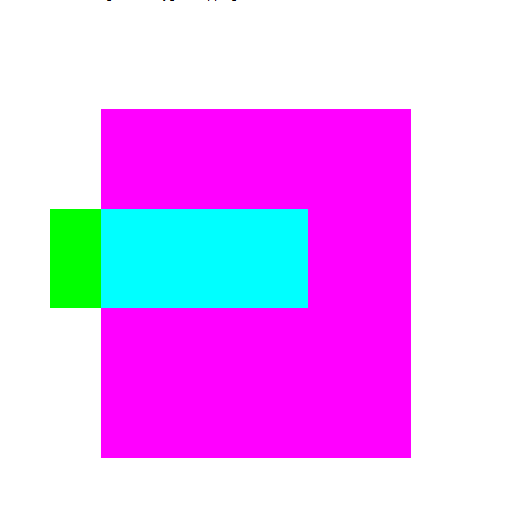
\includegraphics[height=3.5in,width=4in]{polygon_clip}
	\caption{Sutherland-Hodgeman polygon clipping}
\end{figure*}

\section{Discussion}
\begin{enumerate}[(i)]
	\item Sutherland–Hodgman algorithm clips a polygon with extra edges in the viewport. To remove this edge we have to use Weller Atherton algorithm. 
	\item We have clipped a polygon having 4 edges for implementing the algorithm simply.
	\item We didn't take any user input to execute experiment easily. It can be improved more. 
\end{enumerate}

	
\end{document}